\chapter{Bayesian deconvolution}
\label{chapt:bayesian-deconvolution}

Early stages of the SPHERE-2 analysis attempted to directly estimate the parameters of EAS photons in each PMT (photon count and arrival time distribution) from the recorded signal. However, this approach was unsuccessful due to various reasons. Instead, the idea emerged to perform a complete deconvolution, extracting information about the photon flux at the input of each PMT for every moment in time. This deconvolution process must consider the stochastic properties of the PMT. Similar problems are addressed in other domains, such as spectral measurements \cite{Rhode1993} and image processing \cite{Wipf2013}, where Bayesian statistics proves to be valuable by interpreting probability as a measure of information or confidence in the value of a random variable \cite{Gelman2013}.

\section{Problem setup}

The input signal is a set of $\delta$-functions offsetted in time. We use detector's natural time bins ($12.5$ sec) and assume that within each time bin, $\delta$-functions are distributed almost uniformly. Considering $N$ time bins, our goal is to determine the photon count, denoted as $n_i$, in each time bin $[i-1, i]$ for $i = 1 \ldots N$.

We assume that the PMT behaves as a linear system with a stochastic impulse response function $\tilde{h}(t)$. Each $\delta$-function in the input signal is convolved with an independent sample $h(t) \sim \tilde{h}(t)$. This represents the idea of independent fluctuations in PMT amplification for each electron cascade. We assume that each sample from $\tilde{h}(t)$ is causal ($h(t) = 0$ for $t < 0$) and finite in time ($\exists \tilde{L}$ such that $h(t)(t) = 0, \; t > \tilde{L}$). We refer to this random function, which provides a new sample for each input $\delta$-function, as the system's randomized impulse response (RIR). The problem of statistical deconvolution is formulated in Bayesian terms:

\begin{quote}
	Given the randomized impulse response of the system $\tilde{h}(t)$ and the output signal $s_j, \; j = 1, \ldots, N + L$, find the posterior probability density functions for the values $n_i$, $i = 1, \ldots, N$.
\end{quote}

We use \textit{uninformative} prior $P(\vec{n}) = Const$ and denote likelihood function $\mathcal{L}(\vec{s}, \vec{n}) = P(\vec{s} | \vec{n})$, which yields

\begin{equation}
	\label{eq:bayes-theorem-adapted}
	P(\vec{n} | \vec{s}) = \frac{P(\vec{s} | \vec{n}) \, P(\vec{n})}{P(\vec{s})} \propto \mathcal{L}(\vec{s}, \vec{n})
\end{equation}

\section{Likelihood function}
\label{sec:naive-monte-carlo-likelihood}

The PMT output signal $\vec{s}$ is a sample from a multivariate random variable. Denoting it as $\vec{S}$, we can express $S_j$ it as:

\begin{equation}
	S_j = \sum_{l=0}^{L} C(n_{j-l}, l)
	\label{eq:S-definition-as-random-variable}
\end{equation}

$C(n, l)$ is a random variable that describes the contribution of $n$ $\delta$-functions with a \textit{delay} of $l$ bins. Here we take use RIR constraints.

To study the distribution of $C(n, l)$, Monte Carlo simulations are be employed. By sampling the RIR $h_k(t) \sim \tilde{h}(t)$ and an in-bin time $t_{\text{inbin}} \sim U(0, 1)$, we obtain a sample from $C(1, l) = h_k(l + 1 - t_{\text{inbin}})$. Adding $n$ independent samples from it yields a sample from $C(n, l)$.

Directly sampling $S_j$ to calculate likelihood of a particular $\vec{s}$ is computationally infeasible. We approximate the likelihood function using a multivariate normal distribution. We find this approximation suitable for input intensities as low as 4-5 $\delta$-functions per bin, which corresponds to the background intensity observed in the SPHERE-2 detector.

The multivariate normal distribution is defined by the mean vector $\vec{\mu}$ and the covariance matrix $\Sigma$, which are computed from the input $\vec{n}$ and the RIR $\tilde{h}(t)$.

\begin{equation}
	\Sigma_{ij} = \cov(S_i, S_j) = \sum_{l=0}^{L - (i-j)} \cov(C(n_{i-l}, l), C(n_{i-l}, l + (i-j)))
\end{equation}

\begin{figure}
	\centering
	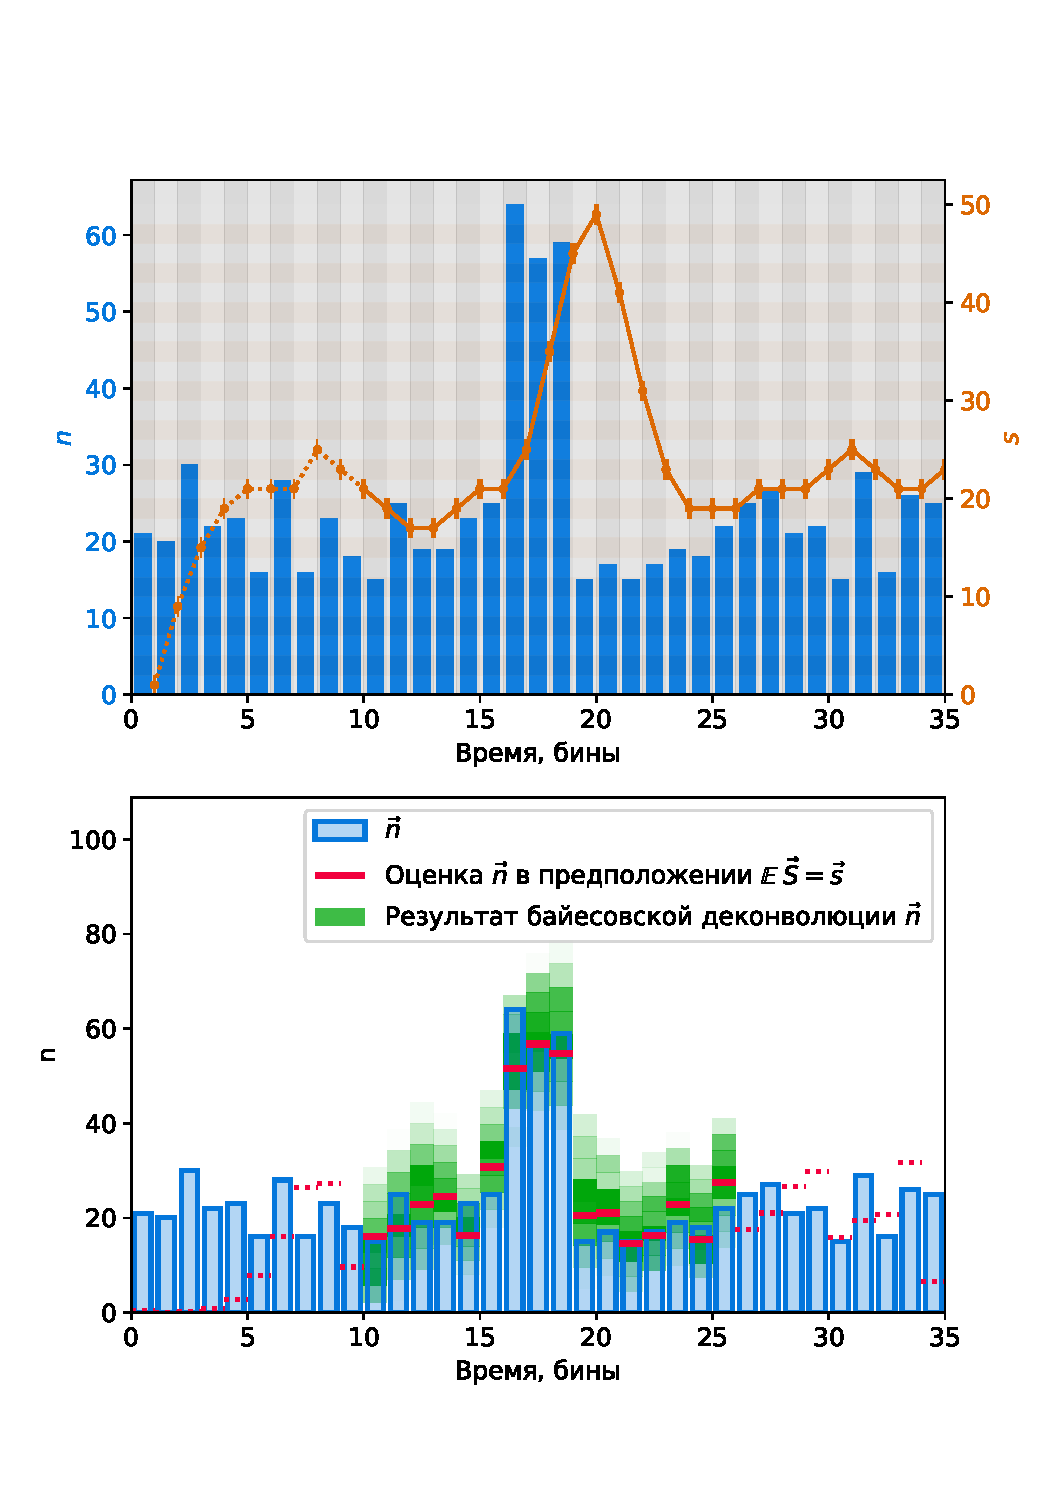
\includegraphics[width=0.85\columnwidth]{final-problem-and-solution}
	\caption{Bayesian deconvolution performed on toy input data. \textbf{Top panel:} toy input data $\vec{n}$ (blue) and corresponding system's output (convolution with SPHERE-2 randomized impulse response) $\vec{s}$, orange (X axis: <<Time, bins>>). \textbf{Bottom pannel}: same input data $\vec{n}$ (blue); rough $\vec{n}$ estimation from mean values, MCMC sampling starting point (red); deconvolution result, marginal posterior distributions in each time bin (green).}
	\label{pic:bayesian-deconvolution-with-experimantal-rir-and-rounding}
\end{figure}


\section{Discretization error}

This approximation assumes precise measurement of the output signal. In reality, the output signal is discretized by ADC. We assume that the ADC rounds down its input, i.e. for each recorded $s_j$, the actual input value lies somewhere between $s_j$ and $s_j + \delta$, following a uniform distribution. To account for this error, we numerically integrate the "exact" likelihood function over an $N$-dimensional cube with side length $\delta$ and a lower corner positioned at $\vec{s}$:


\section{Posterior distribution sampling}
\label{sec:mcmc-sampling}

Using the obtained likelihood function $\mathcal{L}$, we estimate $\vec{n}$ based on the recorded output signal $\vec{s}$ and RIR $\tilde{h}(t)$. Employing Markov Chain Monte Carlo (MCMC) sampling \cite{Sharma2017}, we draw a large sample from $P(\vec{n} | \vec{s}) \propto \mathcal{L}(\vec{n}, \vec{s})$. From this sample of potential $\vec{n}$ values, we obtain the best-fitting input value for the system and its associated error.

For this study, we utilize the affine-invariant MCMC method \cite{Goodman2010} implemented in the Python package emcee \cite{ForemanMackey2016}.

\section{Deconvolution results}

We illustrate deconvolution procedure on toy input data: Poisson background with mean $\lambda=20$ photons per time bin and a <<signal>> photon packet: 3 bins with additional Poisson signal with $\lambda_{\mathrm{signal}}=40$. Fig. \ref{pic:bayesian-deconvolution-with-experimantal-rir-and-rounding} illustrates the system's input and output on the top panel and the deconvolution results on the bottom panel.
